

\begin{frame}{Typical Communication Scenario}
  \vspace{-2ex}
  \begin{center}
  \hfitbox{0.79\linewidth}{%
    \relsize{-2}%
\begin{tikzpicture}
[
  pstep/.style={
    draw=black,
    fill=white,
    line width=0.5pt,
    minimum width=1.5cm,
    minimum height=0.7cm,
    inner sep=0,
    align=center
  },
  hstep/.style={pstep,
    draw=red,
    fill=white,
    line width=0.5pt,
    text=red
  },
  nbox/.style={pstep,
    rectangle
  },
  hbox/.style={hstep,
    rectangle,
  },
  ncloud/.style={pstep,
    cloud,
    cloud puffs=13,
    cloud puff arc=170,
    aspect=2
  },
  hcloud/.style={hstep,
    cloud,
    cloud puffs=13,
    cloud puff arc=170,
    aspect=2
  },
  narrow/.style={
    ->,
    >=latex,
    line width=0.5pt
  },
  harrow/.style={
    ->,
    >=latex,
    line width=0.5pt,
    red
  },
]
  
% %--- just some helper lines for constructing the picture ---
% \draw[gray!20,very thin] (0,0) grid (10,6); 

%==== some defines for perspective projections ====
\def\xx{ 0.75}
\def\xy{ 0.25}
\def\yx{ 0.0}
\def\yy{ 1.0}
\def\zx{-0.1}
\def\zy{ 0.1}


%%%%%%%%%%%%%%%%
%%%
%%%   NODES
%%%
%%%%%%%%%%%%%%%%

%===== scene and capture =====
\node[visible on=<2-|handout:1-3>] (scene) [inner sep=0] at (1,5) {
  \fitbox{2cm}{2cm}{
  \begin{tikzpicture}
    \node [inner sep=0,cm={\xx,\xy,\yx,\yy,(0,0)}] {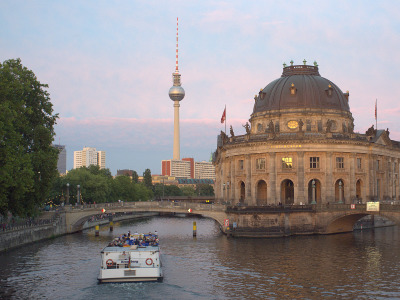
\includegraphics{BerlinBode}};
  \end{tikzpicture}}
};
\node[visible on=<2-|handout:1-3>] (capture) [inner sep=0] at (3,5) {
  \resizebox{!}{2cm}{
  
\begin{tikzpicture}
    % outer area
    \draw[opacity=0.0] (0,0) rectangle (6,12);
    \clip (0,0) rectangle (6,12);
    % camera body
    \draw[fill] (0,5) -- (0,7) -- (1,6.4) 
                {[rounded corners] -- (1,7) -- (5,7) -- (5,5)}
                -- (3.5,5) -- (3.5,5) -- (3.5,4.7) 
                -- (2.5,4.7) -- (2.5,5)
                {[rounded corners] -- (1,5)}
                -- (1,5.6) -- (0,5);
    \draw[fill] (3,4.7) circle [radius=0.5];
    \draw[line width=0.1cm] (3,4.7) -- (4.2,4.3);
    \draw[line width=0.3cm]            (4.2,4.3) -- (4.8,4.1);
    % tripod
    \draw[fill] (2.6,4.1) -- (3.4,4.1) {[rounded corners] -- (3.4,3.0) -- (2.6,3.0) -- (2.6,4.1)};
    \draw[fill] (1.25,0) circle [radius=0.25];
    \draw[fill] (3.00,0) circle [radius=0.25];
    \draw[fill] (4.75,0) circle [radius=0.25];
    \draw[line width=0.2cm] (3,3.2) -- (1.25,0);
    \draw[line width=0.2cm] (3,3.2) -- (3.00,0);
    \draw[line width=0.2cm] (3,3.2) -- (4.75,0);
  \end{tikzpicture}}
};
\node[visible on=<2-|handout:1-3>] at (2.5,5.5) {capture};

%===== raw input data samples =====
\node[visible on=<3-|handout:1-3>] (raw input) [anchor=north,inner sep=0] at (5,6) {
  \resizebox{!}{0.85cm}{
  \begin{tikzpicture}
  [
    b/.style={color=white,fill=gray!10,line width=0},
    g/.style={line width=0.05cm},
    f/.style={line width=0.10cm}
  ]
  \node at ( 0.0,0.0)  {\begin{tikzpicture}
                          \draw[b] (0,0) rectangle (8,6);
                          \draw[g] (0,0) grid      (8,6);
                          \draw[f] (0,0) rectangle (8,6);
                        \end{tikzpicture}};
  \node at (-0.7,0.7)  {\begin{tikzpicture}
                          \draw[b] (0,0) rectangle (8,6);
                          \draw[g] (0,0) grid      (8,6);
                          \draw[f] (0,0) rectangle (8,6);
                        \end{tikzpicture}};
  \node at (-1.4,1.4)  {\begin{tikzpicture}
                          \draw[b] (0,0) rectangle (8,6);
                          \draw[g] (0,0) grid      (8,6);
                          \draw[f] (0,0) rectangle (8,6);
                        \end{tikzpicture}};
  \end{tikzpicture}}
};
\node[visible on=< 3-16|handout:1-2>][align=center]          at (5,4.6) {raw input\\data samples};
\node[visible on=<17-|handout:3>][align=center,text=red] at (5,4.6) {raw input\\data samples};

%===== video encoding =====
\node[visible on=< 4-  |handout:1-3>] (preprocess) [nbox,anchor=north] at (7,6) {pre-\\processing};
\node[visible on=< 5-16|handout:1-2>] (videoenc)   [nbox]              at (9,5) {source\\encoder};
\node[visible on=<17-  |handout:3>] (hvideoenc)  [hbox]              at (9,5) {source\\encoder};

%===== channel =====
\node[visible on=<11-16|handout:1-2>] (transmission) 
[
  rectangle,
  draw=gray,
  fill=gray!10,
  line width=0.5pt,
  minimum width=10.0cm,
  minimum height=1.4cm,
  inner sep=0,
  align=center
]                                                at (5,3)  {};
\node[visible on=<11-16|handout:1-2>] (trans text) 
[
  anchor=north west,
  inner sep=0,
  text=gray
]                                                at (0.1,3.6)
                                                           {transmission channel (can be replaced by storage)};
\begin{scope}[yshift=-0.13cm]
\node[visible on=< 6-16|handout:1-2>] (channelenc)   [nbox]    at (9,3)  {channel\\encoder};
\node[visible on=< 7-16|handout:1-2>] (modulator)    [nbox]    at (7,3)  {modulator};
\node[visible on=< 8-16|handout:1-2>] (channel)      [ncloud]  at (5,3)  {channel};
\node[visible on=< 9-16|handout:1-2>] (demodulator)  [nbox]    at (3,3)  {demodulator};
\node[visible on=<10-16|handout:1-2>] (channeldec)   [nbox]    at (1,3)  {channel\\decoder};
\end{scope}

%===== video decoding =====
\node[visible on=<12-16|handout:1-2>] (videodec)     [nbox]    at (1,1)  {source\\decoder};
\node[visible on=<17-  |handout:3>] (hvideodec)    [hbox]    at (1,1)  {source\\decoder};
\node[visible on=<13-  |handout:1-3>] (postprocess)  [nbox,anchor=south]
                                                   at (3,0)  {post-\\processing};

%===== raw output video samples =====
\node[visible on=<14-|handout:1-3>] (raw output) [anchor=north,inner sep=0] at (5,2) {
  \resizebox{!}{0.85cm}{
  \begin{tikzpicture}
  [
    b/.style={color=white,fill=gray!10,line width=0},
    g/.style={line width=0.05cm},
    f/.style={line width=0.10cm}
  ]
  \node at ( 0.0,0.0)  {\begin{tikzpicture}
                          \draw[b] (0,0) rectangle (8,6);
                          \draw[g] (0,0) grid      (8,6);
                          \draw[f] (0,0) rectangle (8,6);
                        \end{tikzpicture}};
  \node at (-0.7,0.7)  {\begin{tikzpicture}
                          \draw[b] (0,0) rectangle (8,6);
                          \draw[g] (0,0) grid      (8,6);
                          \draw[f] (0,0) rectangle (8,6);
                        \end{tikzpicture}};
  \node at (-1.4,1.4)  {\begin{tikzpicture}
                          \draw[b] (0,0) rectangle (8,6);
                          \draw[g] (0,0) grid      (8,6);
                          \draw[f] (0,0) rectangle (8,6);
                        \end{tikzpicture}};
  \end{tikzpicture}}
};
\node[visible on=<14-16|handout:1-2>] [align=center]          at (5,0.6) {raw output\\data samples};
\node[visible on=<17-  |handout:3>] [align=center,text=red] at (5,0.6) {raw output\\data samples};

%===== display and perception =====
\node[visible on=<15-|handout:1-3>] (display) [inner sep=0] at (7,1) {
  \resizebox{!}{2cm}{
  \begin{tikzpicture}
  [
    x={(\xx cm,\xy cm)},
    y={(\yx cm,\yy cm)},
    z={(\zx cm,\zy cm)}
  ]
  % stand
  \draw [fill,color=black]     (1.0,0.3,-2.5) -- (3.0,0.3,-2.5) -- (3.0,0.1,-2.5) -- (1.0,0.1,-2.5);
  \draw [fill,color=black!50]  (1.0,0.3,-2.5) -- (1.0,0.1,-2.5) -- (1.0,0.1, 3.0) -- (1.0,0.3, 3.5);
  \draw [fill,color=black!70]  (1.0,0.3,-2.5) -- (3.0,0.3,-2.5) -- (3.0,0.3, 3.0) -- (1.0,0.3, 3.5);
  % intermediate
  \draw [fill,color=black]     (1.7,1.0, 0.0) -- (2.3,1.0, 0.0) -- (2.3,0.3, 0.0) -- (1.7,0.3, 0.0);
  \draw [fill,color=black!50]  (1.7,1.0, 0.0) -- (1.7,0.3, 0.0) -- (1.7,0.3, 1.0) -- (1.7,1.0, 1.0);
  % main screen
  \draw [fill,color=black]     (0.0,1.0, 0.0) -- (4.0,1.0, 0.0) -- (4.0,4.0, 0.0) -- (0.0,4.0, 0.0);
  \draw [fill,color=black!50]  (0.0,1.0, 0.0) -- (0.0,4.0, 0.0) -- (0.0,4.0, 1.0) -- (0.0,1.0, 1.0);
  \draw [fill,color=black!70]  (0.0,4.0, 0.0) -- (4.0,4.0, 0.0) -- (4.0,4.0, 1.0) -- (0.0,4.0, 1.0);
  % picture
  \node [inner sep=0,cm={\xx,\xy,\yx,\yy,(0,0)}] at (2.0,2.5) {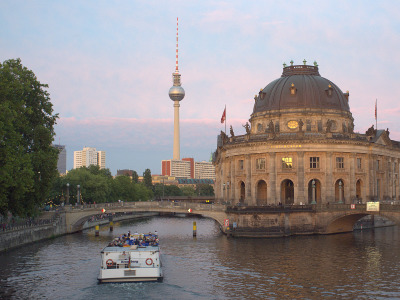
\includegraphics[width=3.6cm]{BerlinBode}};
  \end{tikzpicture}}
};
\node[visible on=<15-|handout:1-3>] (perception) at (9,1) {
  \resizebox{!}{2cm}{
  
\begin{tikzpicture}[
    mline/.style={line width=0.3cm,rounded corners,line cap=round,line join=round}
    ]
    % outer area
    \draw[opacity=0.0] (-2.9,1) rectangle (5.1,12);
    % chair
    \draw[mline] (1.7,3) -- (4,3) -- (4.3,3.2) -- (4.5,3.5) -- (4.8,7);
    \draw[mline] (2.5,3) -- (2.1,1);
    \draw[mline] (3.5,3) -- (3.9,1);
    % man
    \fill (4.5,8.8) circle [x radius=0.7, y radius=1, rotate=-5];
    \draw[mline] (0.3,1) -- (1.2,1) -- (1.2,3.5) -- (3.6,3.5) -- (4.0,4.4) -- (4.4,7.6);
    \draw[mline] (4.2,6.5) -- (3.0,5) -- (1.5,5.9);
    % drink
    \draw[fill] (1.7,6.3) -- (1.9,4.9) -- (2.3,4.9) -- (2.5,6.3);
    \draw[line width=0.1cm] (2.1,6.0) -- (2.5,6.9);
  \end{tikzpicture}
  }
};
\node[visible on=<15-|handout:1-3>] [align=center] at (8.5,1.5) {output and\\perception};


%%%%%%%%%%%%%%%%%%%%%
%%%
%%%   CONNECTIONS
%%%
%%%%%%%%%%%%%%%%%%%%%

%--- raw video input samples
\draw[visible on=< 3-16|handout:1-2>] [narrow] (capture)     -- (videoenc);

%--- preprocess ---
\draw[visible on=< 4-  |handout:1-3>] [fill]   (6,5)            circle [radius=0.03cm];
\draw[visible on=< 4-  |handout:1-3>] [narrow] (6,5)         |- (preprocess);
\draw[visible on=< 4-  |handout:1-3>] [narrow] (preprocess)  -| (8,5);

%--- video encoder ---
\draw[visible on=< 5-16|handout:1-2>] [narrow] (videoenc)    -- (channelenc)
                                                     node [pos=0.35,anchor=east,align=right]
                                                     {encoded\\bitstream};

%--- channel ---
\draw[visible on=< 7-16|handout:1-2>] [narrow] (channelenc)  -- (modulator);
\draw[visible on=< 8-16|handout:1-2>] [narrow] (modulator)   -- (channel);
\draw[visible on=< 9-16|handout:1-2>] [narrow] (channel)     -- (demodulator);
\draw[visible on=<10-16|handout:1-2>] [narrow] (demodulator) -- (channeldec);
\draw[visible on=<10-16|handout:1-2>] [narrow] (channeldec)  -- (videodec)
                                                    node [pos=0.57,anchor=west,align=left] 
                                                    {received\\bitstream};
%--- video decoder ---
\draw[visible on=<12-16|handout:1-2>] [narrow] (videodec)    -- (display);

%--- postprocess ---
\draw[visible on=<13-  |handout:1-3>] [fill]   (2,1)            circle [radius=0.03cm];
\draw[visible on=<13-  |handout:1-3>] [narrow] (2,1)         |- (postprocess);
\draw[visible on=<13-  |handout:1-3>] [narrow] (postprocess) -| (4,1);


%%%%%%%%%%%%%%%%%%%%%%%
%%%
%%%   FINAL ACTIONS
%%%
%%%%%%%%%%%%%%%%%%%%%%%

%----- no transmission errors -----
\node[visible on=<16-16|handout:2>]
     [hcloud,aspect=3,minimum width=3cm] at (5,3)  
{no transmission errors};

%---- without channel ----
\draw[visible on=<17-  |handout:3>] [harrow] (videoenc) |- (5,3) -| (videodec)
                                    node [pos=0,anchor=south,text=red]
                                    {bitstream};
\draw[visible on=<17-  |handout:3>] [harrow] (capture)     -- (hvideoenc);
\draw[visible on=<17-  |handout:3>] [harrow] (hvideodec)   -- (display);

\end{tikzpicture}
  }
\end{center}\vspace{-1.5ex}
\end{frame}
